\documentclass[12pt,a4paper]{article}

\usepackage[utf8]{inputenc}
\usepackage[T1]{fontenc}
\usepackage[francais]{babel}
\usepackage{geometry}
\usepackage{xcolor}
\usepackage{listings}
\usepackage{amsmath}
\usepackage{amssymb}
\usepackage{graphicx}
\usepackage{hyperref}
\usepackage{titlesec}
\usepackage{fancyhdr}
\usepackage{mdframed}
\usepackage{enumitem}
\usepackage{booktabs}
\usepackage{tcolorbox}
\usepackage{parskip}
\usepackage{float}

\geometry{
  top=2.5cm, bottom=2.5cm,
  left=2.8cm, right=2.8cm,
  headheight=15pt
}

%% Couleurs
\definecolor{crtblue}{RGB}{30, 90, 160}
\definecolor{crtgray}{RGB}{245, 245, 248}
\definecolor{crtaccent}{RGB}{220, 60, 40}
\definecolor{crtgreen}{RGB}{40, 140, 80}
\definecolor{crtdark}{RGB}{20, 20, 40}
\definecolor{codebg}{RGB}{250, 250, 253}
\definecolor{codecomment}{RGB}{100, 120, 100}
\definecolor{codekeyword}{RGB}{0, 80, 160}
\definecolor{codestring}{RGB}{160, 30, 30}

%% Style de code C++
\lstdefinestyle{cppstyle}{
  language=C++,
  backgroundcolor=\color{codebg},
  basicstyle=\ttfamily\small,
  keywordstyle=\bfseries\color{codekeyword},
  commentstyle=\itshape\color{codecomment},
  stringstyle=\color{codestring},
  numbers=left,
  numberstyle=\tiny\color{gray},
  numbersep=8pt,
  frame=single,
  framesep=4pt,
  rulecolor=\color{crtblue!30},
  breaklines=true,
  showstringspaces=false,
  tabsize=4,
  captionpos=b,
  xleftmargin=12pt,
  morekeywords={auto, nullptr, override, constexpr, requires, concept, typename, size_t, std},
}
\lstset{style=cppstyle}

%% Boîtes colorées
\tcbuselibrary{skins, breakable}

\newtcolorbox{infobox}[1]{
  colback=crtblue!5,
  colframe=crtblue!60,
  title=#1,
  fonttitle=\bfseries\small,
  breakable,
  before upper=\small
}

\newtcolorbox{warningbox}[1]{
  colback=crtaccent!5,
  colframe=crtaccent!50,
  title=#1,
  fonttitle=\bfseries\small,
  breakable,
  before upper=\small
}

\newtcolorbox{successbox}[1]{
  colback=crtgreen!5,
  colframe=crtgreen!50,
  title=#1,
  fonttitle=\bfseries\small,
  breakable,
  before upper=\small
}

%% En-têtes et pieds de page
\pagestyle{fancy}
\fancyhf{}
\fancyhead[L]{\small\textcolor{gray}{Rapport de soutenance - Enzo Chen - Aurélie Mordice - Milena Catin de Gouttes Lastouzeilles}}
%\fancyhead[R]{\small\textcolor{crtblue}{Simulateur de circuits analogiques}}
\fancyfoot[C]{\small\textcolor{gray}{\thepage}}
\renewcommand{\headrulewidth}{0.4pt}
\renewcommand{\headrule}{\hbox to\headwidth{\color{crtblue}\leaders\hrule height \headrulewidth\hfill}}

%% Titres de sections
\titleformat{\section}[block]
  {\Large\bfseries\color{crtblue}}
  {\thesection}{1em}{}

\titleformat{\subsection}[block]
  {\large\bfseries\color{crtdark}}
  {\thesubsection}{1em}{}

\titleformat{\subsubsection}[block]
  {\normalsize\bfseries\color{crtdark}}
  {\thesubsubsection}{1em}{}

%% Liens hypertexte
\hypersetup{
  colorlinks=true,
  linkcolor=crtblue,
  urlcolor=crtblue,
  citecolor=crtgreen,
  pdftitle={Rapport de soutenance -- Simulateur de circuits analogiques en C++},
  pdfauthor={},
}

%%────────────────────────────────────────────────────────
\begin{document}

%%── PAGE DE TITRE ─────────────────────────────────────────
\begin{titlepage}
  \pagecolor{crtblue}
  \color{white}
  \vspace*{3cm}

  \begin{center}
  

    {\fontsize{36}{40}\selectfont\bfseries Simulateur de circuits\\[6pt] analogiques en C++}\\[1.2cm]

    \textcolor{white!70}{\rule{10cm}{0.5pt}}\\[1.2cm]

    {\large Rapport de soutenance --- Projet de 1\textsuperscript{re} année}\\[2cm]

    \begin{tcolorbox}[
      colback=white!15, colframe=white!40,
      width=9cm, arc=4pt,
      boxrule=0.5pt,
      left=12pt, right=12pt, top=10pt, bottom=10pt
    ]
      \centering
      \textbf{Auteurs}\\[6pt]
      Enzo Chen \\ Aurélie Mordice \\ Milena Catin de Gouttes Lastouzeilles\\[8pt]
      
    \end{tcolorbox}

    \vfill
    {\small Mai 2026}
  \end{center}
\end{titlepage}
\nopagecolor

%%── TABLE DES MATIÈRES ─────────────────────────────────────
\newpage
\tableofcontents
\newpage

%%════════════════════════════════════════════════════════════
\section{Introduction et vision du projet}
%%════════════════════════════════════════════════════════════

\subsection{Le problème adressé}

Analyser le comportement d'un circuit électronique analogique demande normalement soit
du matériel physique (oscilloscope, alimentation, composants), soit un logiciel commercial
lourd (SPICE, LTspice). L'objectif de ce projet est de proposer une bibliothèque C++ légère et 
extensible permettant de simuler numériquement l'état d'équilibre d'un circuit
à partir de ses composants et de leurs connexions.

\subsection{Principe général de la simulation}

Un circuit électronique en régime continu vérifie la loi des nœuds ou \textbf{Première loi de Kirchhoff} : 
la somme algébrique des courants entrant dans chaque nœud est égale à la somme algébrique des courants sortant de ce nœud. 
Chaque composant vérifie aussi leur \textbf{loi tension-courant} : la relation entre la tension aux bornes d'un composant et le courant qui le traverse.

Notre bibliothèque \texttt{crt} modélise ce problème comme un \textbf{problème d'optimisation} :
on cherche les potentiels $V_1, \ldots, V_n$ sur les fils du circuit qui minimisent l'erreur totale

\[
  E(V_1, \ldots, V_n) = \sum_{w \in \text{fils libres}} \left(\sum_{p \in \text{pins}(w)} I_p(V_1, \ldots, V_n)\right)^2
\]

où $I_p(V_1, \ldots, V_n)$ est le courant calculé par le composant associé au nœud (pin) $p$ en fonction des potentiels des fils.
Quand $E = 0$ (ou s'en rapproche le plus possible), la loi des nœuds est vérifiée en tout nœud : le circuit est résolu.

\begin{infobox}{Pourquoi une formulation par optimisation ?}

  Cette formulation présente une certaine flexible : elle permet d'ajouter n'importe quel composant (diode, transistor...) en définissant 
  simplement sa loi $I(V)$ et sa dérivée $dI/dV$.
  C'est un choix extensible, au prix d'une convergence parfois plus lente
  que les méthodes directes.

\end{infobox}


%%════════════════════════════════════════════════════════════
\section{Architecture du projet}
%%════════════════════════════════════════════════════════════


Les circuits électroniques que l'on simule sont composés de :
\begin{itemize}
    \item Components (composants de la simulation : Résistance, Transistor, Diode)
    \item Wires (Fils)
    \item Const\_Wires (Fils dont la valeur de potentiel est constante)
    \item Pins (interface entre un composant et un fils)
    \item Circuit naïf (Contient des fils et des composants)
    \item Circuit gradient
\end{itemize}

\subsection{Vue d'ensemble des fichiers}

\begin{center}
\begin{tabular}{lp{9cm}}
  \toprule
  \textbf{Fichier} & \textbf{Rôle} \\
  \midrule
  \texttt{crtDefs.hpp}       & Types fondamentaux : \texttt{Pin}, \texttt{Wire\_ref}, \texttt{Component\_ref} \\
  \texttt{crtWire.\{hpp,cpp\}}       & Nœuds du circuit (fils libres et fils fixes) \\
  \texttt{crtComponent.hpp}  & Interface abstraite \texttt{Component} et template \texttt{Comp<N>} \\
  \texttt{crtResistor.\{hpp,cpp\}}   & Modèle résistance linéaire \\
  \texttt{crtDiode.\{hpp,cpp\}}      & Modèle diode (équation de Shockley) \\
  \texttt{crtTransistor.\{hpp,cpp\}} & Modèle transistor (équation d'Ebers-Moll) \\
  \texttt{crtCircuit.\{hpp,cpp\}}    & Conteneur circuit, calcul de l'erreur totale \\
  \texttt{crtCircuitGrad.\{hpp,cpp\}}& Extension avec calcul du gradient analytique \\
  \texttt{crtConcept.hpp}    & Concepts C++20 pour la vérification statique de types \\
  \texttt{crtSolver.hpp}     & Solveurs (descente de gradient, résolution naïve) \\
  \texttt{crtUtilities.\{hpp,cpp\}}  & Export GraphViz / visualisation \\
  \bottomrule
\end{tabular}
\end{center}

\subsection{Hiérarchie des types}

\begin{verbatim}
Wire_ref : shared_ptr sur un wire.
Pin_ref : shared_ptr sur un pin.
Component_ref : shared_ptr sur un component.

Component (interface abstraite)
  +-- Comp<NB_PINS>   (gère le nombre de pins dans les composants)
        +-- Resistor  (2 pins, loi d'Ohm)
        +-- Diode     (2 pins, équation de Shockley)
        +-- Transistor(3 pins, modèle Ebers-Moll)

Wire (noeud de potentiel libre)
  +-- Const_Wire  (potentiel imposé, non modifiable)

Circuit
  +-- vector<Wire_ref>       -- fils libres
  +-- vector<Wire_ref>       -- fils fixes (const_wires)
  +-- vector<Component_ref>  -- composants

GradCircuit : Circuit (hérite de Circuit)
  +-- compute_grad() -- gradient analytique de l'erreur
\end{verbatim}

\begin{figure}[H]
    \centering
    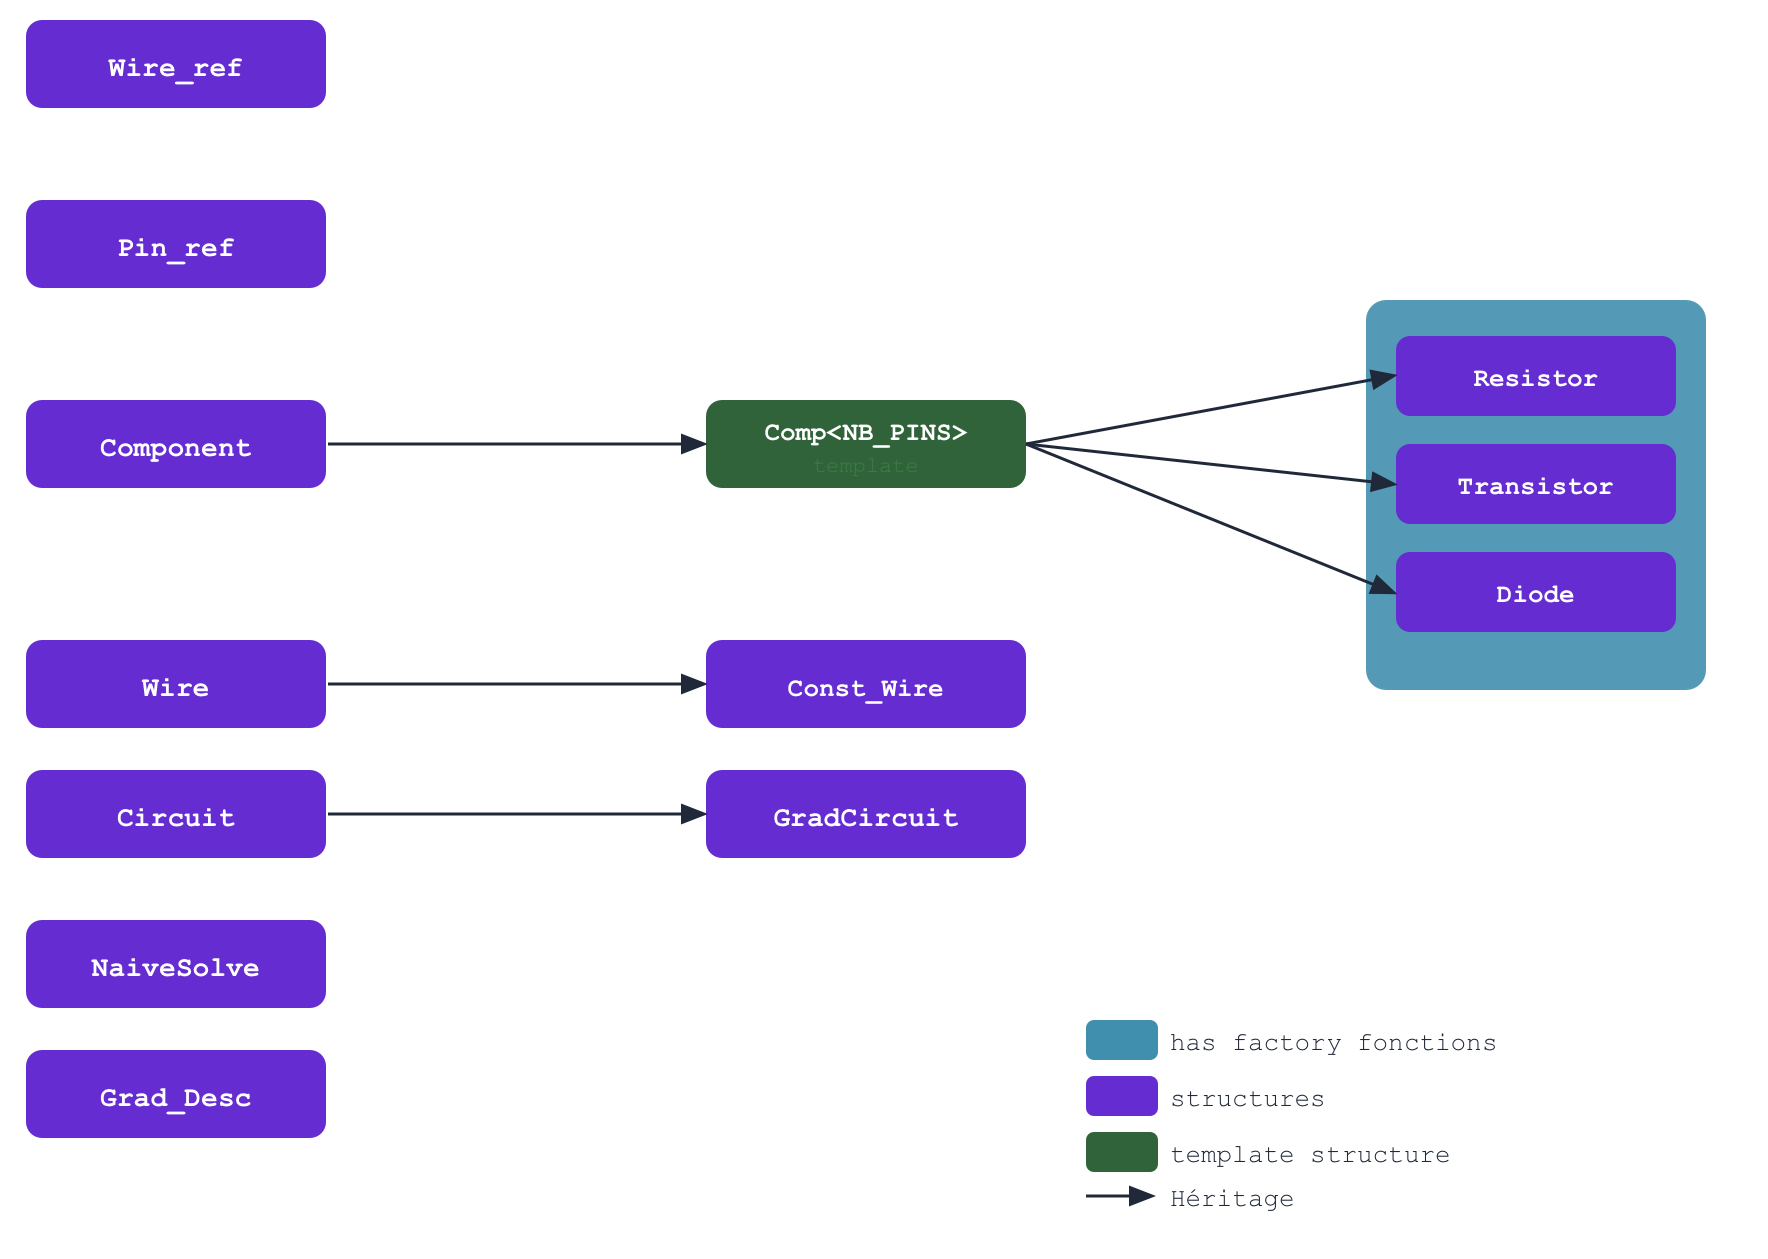
\includegraphics[width=\textwidth]{pics/schema_inheritance_white.png}
    \caption{Vision d'ensemble de l'architecture de notre projet.}
    \label{fig:exemple}
\end{figure}


\subsection{Modélisation}

\noindent
La diode est modélisée par le \textbf{l'équation de Shockley} :
\[ I_D = I_s \left( \exp^{\frac{V_D}{n V_T}} - 1 \right) \]
Avec :
  \begin{itemize}
    \item \( I_D \) courant traversant la diode,
    \item \(I_S = 1 \cdot 10^{-12}\ A\) courant de saturation pris à 27 \textdegree C,
    \item \( V_D \) la tension aux bornes de la diode,
    \item \( V_T = 25.852\ mV\) le potentiel thermique pris à 27 \textdegree C,
    \item \( n = 1\) facteur de qualité idéal.
  \end{itemize}


Nous avons choisi ces paramètres pour la diode afin de représenter le composant à température ambiante. L'utilisateur ne peut
pas changer ces caractéristiques car nous avons choisi de ne pas implémenter l'influence de la température sur la diode. Nous avons fait ce choix de conception pour l'efficacité et la simplicité. De même pour le transistor.

\noindent
Le transistor est modélisé par \textbf{l'équation d'Ebers-Moll} : 
\[ I_E = I_{ES} \left( \exp^{\frac{V_{BE}}{ V_T}} - 1 \right) \text{,}\quad
 I_C = \alpha_F I_E \quad \text{et} \quad I_B = \left ( 1 - \alpha_F \right ) I_E\] \\
 
Avec : 
\begin{itemize}
  \item \( I_E \) le courant émis par le transistor,
  \item \( I_C \) le courant collecteur,
  \item \( I_B \) le courant de base,
  \item \(I_{ES} = 1 \cdot 10^{-12}\ A\) courant de saturation pris à 27\textdegree C,
  \item \( V_{BE} \) la tension aux bornes du transistor entre le point B et le point E,
  \item \( V_T = 25.852\ mV\) le potentiel thermique pris à 27\textdegree C,
  \item \( \alpha_F = 0.98\) le gain de courant .
\end{itemize}



%%════════════════════════════════════════════════════════════
\section{Partie utilisateur : construire et connecter un circuit}
%%════════════════════════════════════════════════════════════

\subsection{Créer des fils et des composants}

L'API est pensée pour être la plus lisible possible. Voici comment construire un
circuit simple : une résistance et une diode en série alimentées par 5 V.

\begin{lstlisting}[caption={Exemple d'utilisation : circuit résistance + diode}]
#include <crt.hpp>

int main()
{
    crt::GradCircuit c;
    auto r{c += crt::make::resistor(10)};
    auto d{c += crt::make::diode()};
    auto [vcc, gnd] = c.make_generator(10);
    auto mid = c.wire();

    vcc == r->pin<0>(); 
    mid == r->pin<1>();
    mid == d->pin<0>(); 
    gnd == d->pin<1>();
    solve<Grad_Desc>(c);
    return 0;
}
\end{lstlisting}

\clearpage

\subsection{La surcharge \texttt{operator==} : un choix de conception}

La connexion entre un fil et une broche utilise la surcharge de \texttt{operator==} :

\begin{lstlisting}[caption={Surcharge de == pour la connexion (crtWire.hpp)}]
inline void operator==(Wire_ref w, Pin_ref p)
{
    w->pins.push_back(p);  // le fil connait ses broches
    p->wire = w;           // la broche connait son fil
}
\end{lstlisting}

Ce choix rend la syntaxe de câblage proche d'un schéma électrique naturel (\texttt{fil == broche}).
Cependant ce choix peut-être discutable (voir section~\ref{sec:critique}) car \texttt{operator==}
retourne normalement un booléen.

\subsection{Génération de la vue graphique}

Le circuit peut être exporté au format GraphViz (DOT) pour être visualisé :

\begin{lstlisting}[caption={Export GraphViz}]
#include <crtUtilities.hpp>
#include <fstream>

std::ofstream dot("circuit.dot");
dot << circuit;
dot.close();
crt::utilities::show("circuit.dot"); // genere et ouvre le PDF
\end{lstlisting}

%%════════════════════════════════════════════════════════════
\section{Les Solveurs}
%%════════════════════════════════════════════════════════════

\subsection{Solveur naïf (\texttt{NaiveSolve})}

Le solveur naïf explore chaque fil indépendamment et tente de réduire l'erreur
par tâtonnement numérique :

\begin{lstlisting}[caption={Bouble principale du solveur naïf (crtSolver.hpp)}]
for (auto it = c.wires.begin(); it < c.wires.end(); ++it)
{
    auto w = *it;
    double oldV = w->get_potential();

    w->set_potential(oldV + epsilon);
    double err_plus = c.compute_total_error();
    w->set_potential(oldV - epsilon);
    double err_minus = c.compute_total_error();

    w->potential = (err_plus < err_minus)
                 ? oldV + epsilon
                 : oldV - epsilon;
}
\end{lstlisting}

Il évalue deux perturbations symétriques ($V \pm \varepsilon$) et choisit
la direction qui réduit l'erreur totale. Simple à implémenter, il souffre de
plusieurs limitations :
\begin{itemize}
  \item Chaque fil est traité séquentiellement, sans coordination globale.
  \item Le pas $\varepsilon = 10^{-6}$ est fixe : trop grand, il oscille ;
        trop petit, il converge lentement.
  \item La complexité est $\mathcal{O}(N_{\text{fils}} \times k_{\text{iter}})$
        avec un nombre d'itérations potentiellement très grand.
\end{itemize}

Une améliorer possible de ce solveur serait de modifier la méthode de sélection des fils : il serait 
plus judicieux de choisir un fil aléatoirement dans le circuit et de lui ajouter ou retirer $\varepsilon$ au lieu de parcourir
chaque fil dans un ordre donné.

\subsection{Solveur par descente de gradient (\texttt{Grad\_Desc})}

\subsubsection{La fonction d'erreur et son gradient}

L'erreur totale est :
\[
  E(\mathbf{V}) = \sum_{w} \left(\text{err}(w)\right)^2, \quad
  \text{err}(w) = \sum_{p \in \text{pins}(w)} I_p
\]

Son gradient par rapport au potentiel $V_i$ d'un fil $i$ est :
\[
  \frac{\partial E}{\partial V_i}
  = 2 \sum_{w} \text{err}(w)
    \underbrace{\sum_{p \in \text{pins}(w)} \frac{\partial I_p}{\partial V_i}}_{\partial\,\text{err}(w)/\partial V_i}
\]

Chaque composant doit donc implémenter la méthode \texttt{d(wire\_ref, pin\_ref)} qui retourne la valeur de 
$\partial I_p / \partial V_i$ évaluée en les potentiels actuels et nous allons détailler le calcul de ces dérivées dans les parties suivantes.

\subsubsection{Calcul de la dérivée pour la résistance}

On définit l'expression $pin\_in$ pour le noeud où l'intensité entre dans le composant ($pin\ 0$) et l'expression
$pin\_out$ pour le noeud où l'intensité sort du composant ($pin\ 1$).

Pour une résistance $R$ connectée entre 2 fils de potentiels $V_1$ et $V_2$ :
\[
  I_{\text{pin\_in}} = -\frac{V_1 - V_2}{R}, \qquad I_{\text{pin\_out}} = +\frac{V_1 - V_2}{R}
\]

Ainsi si l'on dérive par rapport à $V_1$ :
\[
  \frac{\partial I_{\text{pin\_in}}}{\partial V_1} = -\frac{1}{R}, \qquad \frac{\partial I_{\text{pin\_out}}}{\partial V_1} = \frac{1}{R}
\]

Si l'on dérive par rapport à $V_2$ :
\[
  \frac{\partial I_{\text{pin\_in}}}{\partial V_2} = \frac{1}{R}, \qquad \frac{\partial I_{\text{pin\_out}}}{\partial V_2} = -\frac{1}{R}
\]

Sinon, les dérivées sont nulles car les intensités ne dépendent que de $V_1$ et de $V_2$.


\subsubsection{Calcul de la dérivée pour la diode}

La diode suit l'équation de Shockley : $I_D = I_S(e^{U/V_T} - 1)$, avec $U = V_1 - V_2$ et $V_1$, $V_2$ les potentiels des fils connectés.

Pour une diode connectée entre les fils de potentiels $V_1$ et $V_2$ :
\[
  I_{\text{pin\_in}} = - I_D, \qquad I_{\text{pin\_out}} = + I_D
\]

Ainsi, les dérivées par rapport à $V_1$ sont : 
\[
  \frac{\partial I_{\text{pin\_in}}}{\partial V_1} = -\frac{I_S}{V_T} e^{U/V_T}, \qquad \frac{\partial I_{\text{pin\_out}}}{\partial V_1} = \frac{I_S}{V_T} e^{U/V_T}
\]

Les dérivées par rapport à $V_2$ sont :
\[
  \frac{\partial I_{\text{pin\_in}}}{\partial V_2} = \frac{I_S}{V_T} e^{U/V_T}, \qquad \frac{\partial I_{\text{pin\_out}}}{\partial V_2} = -\frac{I_S}{V_T} e^{U/V_T}
\]

De même, la dérivée par rapport aux autres potentiels est nulle. 

\subsubsection{Calcul de la dérivée pour le transistor}

Le transistor suit l'équation d'Ebers-Moll, celui-ci est connecté à 3 fils de potentiels respectifs $V_B$, $V_E$ et $V_C$ :
\[ I_E = I_{ES} \left( e^{\frac{V_{BE}}{ V_T}} - 1 \right)\]
\[ I_C = \alpha_F I_E\]
\[ I_B = \left ( 1 - \alpha_F \right ) I_E\]

Avec $V_{BE} = V_B - V_E$

Ainsi, les dérivées par rapport à $V_B$ sont : 
\[
  \frac{\partial I_E}{\partial V_B} = \frac{I_{ES}}{V_T} e^{V_{BE}/V_T}, \qquad \frac{\partial I_B}{\partial V_B} = (1 - \alpha_F) \frac{\partial I_E}{\partial V_B}, 
  \qquad \frac{\partial I_C}{\partial V_B} = \alpha_F \frac{\partial I_E}{\partial V_B} 
\]

Les dérivées par rapport à $V_E$ sont :
\[
  \frac{\partial I_E}{\partial V_E} = - \frac{I_{ES}}{V_T} e^{V_{BE}/V_T}, \qquad \frac{\partial I_B}{\partial V_E} = (1 - \alpha_F) \frac{\partial I_E}{\partial V_E}, 
  \qquad \frac{\partial I_C}{\partial V_E} = \alpha_F \frac{\partial I_E}{\partial V_E} 
\]

Sinon, les dérivées par rapport aux autres potentiels sont nulles car les intensités dépendent uniquement de $V_E$ et de $V_B$.

\subsubsection{Stratégie de pas adaptatif}

La descente de gradient naïve avec pas fixe diverge facilement sur des composants
non linéaires (l'exponentielle de la diode ou du transistor peut exploser). Le solveur implémente
donc un pas adaptatif :

\begin{lstlisting}[caption={implémentation du pas adaptatif (crtSolver.hpp)}]
double local_step = step;
while (local_step > 1e-15)
{
    // Appliquer le pas candidat
    for (auto w : all_wires)
        if (!w->is_fixed())
            w->set_potential(old_pot[j] - local_step * g[j]);

    double new_error = c.compute_total_error();

    if (new_error < old_error - 1e-15) {
        accepted = true;
        break;            // bonne direction et bon pas
    }

    // Reinitialiser et reduire le pas
    restore_potentials();
    local_step *= 0.95;
}
\end{lstlisting}

Le pas est réduit de 5\,\% à chaque échec jusqu'à trouver un pas acceptable ou
descendre sous le seuil $10^{-15}$, ce qui interrompt la résolution.


\subsection{Comparaison des deux solveurs}

\begin{center}
\begin{tabular}{lcc}
  \toprule
  \textbf{Critère} & \textbf{NaiveSolve} & \textbf{Grad\_Desc} \\
  \midrule
  Nécessite \texttt{compute\_grad()} & Non & Oui \\
  Gère les non-linéarités & Peu & Bien \\
  Convergence & Lente & Rapide \\
  Robustesse & Moyenne & Moyenne \\
  Extensibilité & Facile & Requiert $\partial I / \partial V$ \\
  \bottomrule
\end{tabular}
\end{center}

\begin{infobox}{Quand utiliser quel solveur ?}
  Le solveur naïf est utile pour vérifier un circuit purement résistif ou
  pour déboguer un nouveau composant (pas besoin d'implémenter \texttt{d()}).
  La descente de gradient est recommandée pour sa rapidité.
\end{infobox}

\subsection{Analyse de la stagnation}
 
Pour comprendre pourquoi les deux solveurs peinent à converger sur un circuit
contenant une diode, on peut visualiser le graphe de l'erreur quadratique sur un circuit contenant
2 résistances et une diode en série (figure \ref{fig:courbe1}).

\begin{figure}
    \centering
    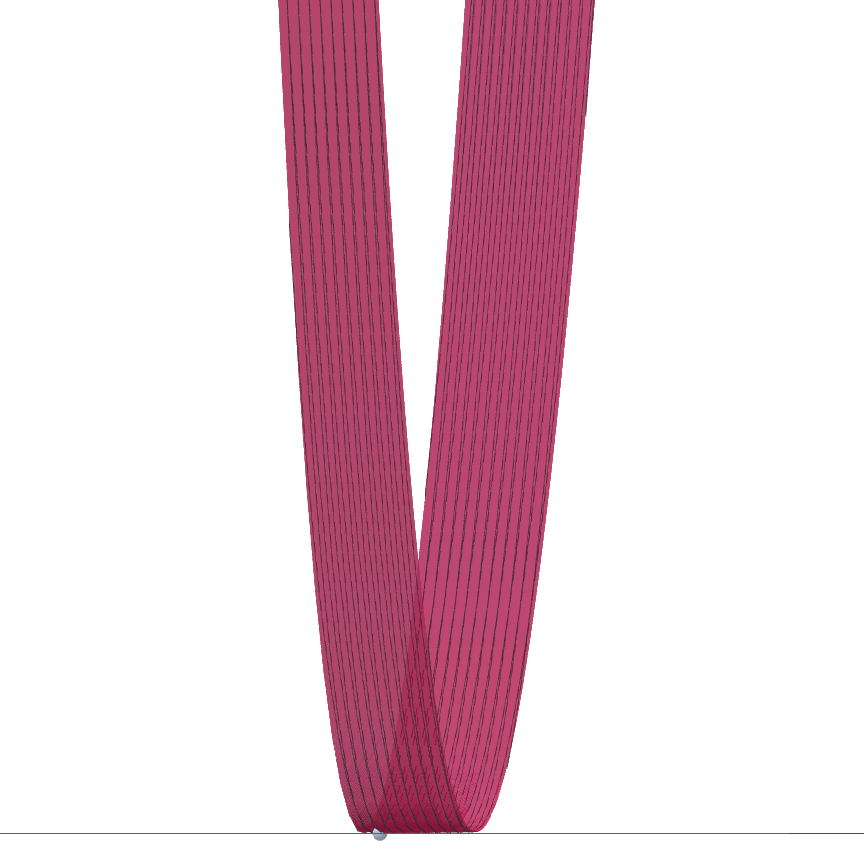
\includegraphics[width=0.6\linewidth]{pics/courbe_erreur_quad1.png}
    \caption{Vue du graphe de l'erreur quadratique avec une ligne horizontale représentant le zéro.}
    \label{fig:courbe1}
\end{figure}

Cette courbe suit l'équation suivante : 
\begin{equation*}
    E(V_3, V_4) = \left(\frac{E_g - V_3}{R_1} - I_s\left(e^{\frac{V_3-V_4}{V_T}}-1\right)\right)^2 
    + \left(I_s\left(e^{\frac{V_3-V_4}{V_T}}-1\right) - \frac{V_4}{R_2}\right)^2
\end{equation*}
Avec :
\begin{itemize}
    \item \( E_g = 10V = V_1-V_2\) tension du générateur avec \(V_2\) potentiel de la masse,
    \item \( R_1 = 10\ \Omega\),
    \item \(R_2 = 5\ \Omega\),
    \item \( I_s = 10^{-12}\ \text{A}\),
    \item \( V_T = 0{,}02585\ \text{V}\).
  \end{itemize}
 
\subsubsection{Stagnation du solveur naïf}
 
Le solveur naïf teste, indépendamment pour chaque potentiel, deux perturbations symétriques $V_i \pm \varepsilon$ et
choisit la direction qui réduit $E$. Dans la zone plate de la vallée
(figure~\ref{fig:courbe1}), les deux erreurs vérifient :
\[
  E(V_i + \varepsilon) \approx E(V_i - \varepsilon) \quad\text{ avec} \quad i \in \{3,4\} 
\]
La différence est inférieure à la précision numérique du \texttt{double}.
Le solveur ne peut plus discriminer de direction préférentielle et oscille
sans progresser. En termes géométriques : \textbf{le gradient numérique d’ordre 1 ne permet plus 
de distinguer une direction de descente significative}.
 
\subsubsection{Stagnation de la descente de gradient}
 
La descente de gradient est bloquée par la \textbf{Zone plate : critère d'arrêt prématuré et échec du pas adaptatif.}
Dans la vallée large (figure~\ref{fig:courbe1}), l'erreur quadratique
décroît très lentement. Elle peut atteindre le seuil de tolérance
$10^{-12}$ \emph{avant} d'avoir atteint le fond, car la surface de l'erreur est si peu courbée
que le gradient est numériquement indiscernable de zéro loin du minimum réel.
Le solveur est géométriquement «~coincé~» au bord du creux sans pouvoir
y entrer.


%%════════════════════════════════════════════════════════════
\section{Les concepts C++20 : contrats à la compilation}
%%════════════════════════════════════════════════════════════

Un des points techniques les plus soignés du projet est l'utilisation des
\textbf{concepts C++20} pour vérifier statiquement qu'un circuit passé à un solveur
possède toutes les méthodes requises.

\begin{lstlisting}[caption={Concept Grad\_Desc (crtConcept.hpp)}]
template <typename Circuit>
concept Grad_Desc =
    NaiveSolve_Circuit<Circuit> &&   // herite du concept naif
    requires(Circuit c) {
        { c.compute_grad() } -> std::ranges::range;
        { *(c.compute_grad().begin()) } -> std::convertible_to<double>;
    };
\end{lstlisting}

Si l'utilisateur passe un \texttt{Circuit} (sans \texttt{compute\_grad()}) au
solveur par gradient, le compilateur émet un message d'erreur clair :

\begin{verbatim}
error: crt::Concept::Grad_Desc is not satisfied.
       use crt::GradCircuit or another class with methode compute_grad().
\end{verbatim}

Cela évite des erreurs de linkage cryptiques et documente l'API par des
contraintes vérifiables.

%%════════════════════════════════════════════════════════════
\section{Analyse critique des choix de conception}
\label{sec:critique}
%%════════════════════════════════════════════════════════════

\subsection{Ce qui fonctionne bien}

\begin{successbox}{Points forts de l'architecture}
\begin{itemize}
  \item \textbf{Extensibilité} : ajouter un nouveau composant ne nécessite que
        d'hériter de \texttt{Comp<N>} et d'implémenter \texttt{compute\_i()},
        \texttt{d()}, \texttt{name()} et \texttt{symbol()}.
  \item \textbf{Séparation solveur/circuit} : les solveurs sont des structs
        indépendants qui opèrent sur n'importe quel circuit vérifiant le concept
        approprié. On peut changer de solveur sans toucher au circuit.
  \item \textbf{Concepts C++20} : les erreurs de typage sont détectées à la
        compilation avec des messages compréhensibles.
  \item \textbf{Polymorphisme par \texttt{shared\_ptr}} : la gestion mémoire est
        automatique, sans risque de fuite ou de double libération.
\end{itemize}
\end{successbox}

\subsection{Choix discutables}

\begin{warningbox}{Points d'amélioration de conception}
\begin{itemize}
  \item \textbf{Surcharge de \texttt{operator==} pour la connexion} : retourner
        \texttt{void} sur un opérateur attendu booléen est surprenant et peut
        dérouter un lecteur. Une méthode \texttt{connect(wire, pin)} serait plus
        explicite et idiomatique.
  \item \textbf{Attribut \texttt{potential} public dans \texttt{Wire}} : le
        potentiel est directement accessible en écriture (\texttt{w->potential = ...})
        dans \texttt{NaiveSolve}, contournant ainsi l'encapsulation de
        \texttt{set\_potential()}. Un accesseur uniforme serait préférable.
  \item \textbf{Gradient calculé sur les fils fixes aussi} : \texttt{GradCircuit::compute\_grad()}
        calcule le gradient pour \texttt{all\_wires} (libres et fixes), mais
        le solveur n'applique les mises à jour qu'aux fils libres. Le code est
        correct mais légèrement redondant en calcul.
  \item \textbf{Pas de tests unitaires} : l'absence de cas de test formels (valeurs
        attendues connues analytiquement) rend difficile la détection de
        régressions lors de modifications.
  \item \textbf{Pas d'influence thermique} : La diode et le transistor possèdent des caractéristiques
        qui dépendent de la température. Or, nous n'avons pas pris cela en compte.
\end{itemize}
\end{warningbox}

%%════════════════════════════════════════════════════════════
\section{Ce que nous aurions aimé ajouter}
%%════════════════════════════════════════════════════════════

\subsection{Solveur de Newton--Raphson}

La méthode de Newton--Raphson est l'algorithme standard des simulateurs de
circuits. Elle converge quadratiquement alors que la
descente de gradient converge linéairement.

Le système à résoudre est $\mathbf{f}(\mathbf{V}) = \mathbf{0}$, où
$f_w = \sum_p I_p$ est l'équation de nœud pour le fil $w$.
La méthode de Newton itère :

\[
  \mathbf{J} \cdot \Delta\mathbf{V} = -\mathbf{f}(\mathbf{V}^{(k)}),
  \qquad \mathbf{V}^{(k+1)} = \mathbf{V}^{(k)} + \Delta\mathbf{V}
\]

où $J_{ij} = \partial f_i / \partial V_j$ est la \textbf{matrice jacobienne},
qui regroupe exactement les dérivées \texttt{d(wire, pin)} déjà calculées dans
le projet. L'infrastructure est donc presque complète pour implémenter Newton :
il manque uniquement l'assemblage de $\mathbf{J}$ et la résolution du système
linéaire $\mathbf{J}\Delta\mathbf{V} = -\mathbf{f}$ (par exemple via Eigen ou
une décomposition LU maison).

\begin{lstlisting}[caption={Pseudo-code Newton-Raphson (non implementé)}]
// Assembler le Jacobien J et le vecteur f
for (size_t i = 0; i < free_wires.size(); ++i)
    for (size_t j = 0; j < all_wires.size(); ++j)
        for (auto p : all_wires[i]->pins)
            J[i][j] += p->component->d(all_wires[j], p);

// Resoudre J * dV = -f  (LU ou conjugate gradient)
auto dV = linear_solve(J, -f);

// Mise a jour des potentiels
for (size_t i = 0; i < free_wires.size(); ++i)
    free_wires[i]->set_potential(V[i] + dV[i]);
\end{lstlisting}

\subsection{Autres extensions envisagées}

\begin{itemize}
  \item \textbf{Simulation en régime transitoire} : introduire une dépendance
        temporelle et modéliser condensateurs et bobines.
  \item \textbf{Interface utilisateur} : remplacer la sortie DOT/GraphViz par
        une représentation schématique standard.
  \item \textbf{Tests unitaires} : valider chaque composant sur des circuits
        dont la solution analytique est connue (diviseur de tension, redresseur
        idéal, etc.).
  \item \textbf{Influence thermique} : rajouter l'influence de la température dans
  les caractéristiques de la diode et du transistor.
\end{itemize}

%%════════════════════════════════════════════════════════════
\section{Ce qui ne s'est pas bien passé}
%%════════════════════════════════════════════════════════════

\begin{itemize}
  \item \textbf{Convergence instable de la diode} : l'exponentielle de l'équation
        de Shockley peut atteindre des valeurs astronomiques pour de grandes tensions.
        Plusieurs tentatives de clamping ($U_{\max} = 0.5\,\text{V}$) ont été essayées
        puis abandonnées car elles introduisaient des discontinuités dans le gradient.
        Le backtracking atténue ce problème sans le résoudre fondamentalement.

  \item \textbf{Gestion des cas dégénérés} : un circuit mal câblé (composant
        connecté à aucun fil) ne génère pas d'erreur explicite mais produit
        des résultats silencieusement incorrects.

  \item Nos 2 solvers ne parviennent pas à converger vers une solution en cas de \texttt{"plateau"} dans la fonction de l'erreur quadratique. 
\end{itemize}

%%════════════════════════════════════════════════════════════
\section{Guide de reprise du projet}
%%════════════════════════════════════════════════════════════

\subsection{Prérequis}

\begin{itemize}
  \item Compilateur C++ avec support C++20 (\texttt{g++ >= 12} ou \texttt{clang++ >= 14}).
  \item Option de compilation : \texttt{-std=c++20 -I<chemin\_vers\_headers>}.
  \item Optionnel : \texttt{neato} (paquet \texttt{graphviz}) pour la visualisation.
\end{itemize}

\subsection{Ajouter un nouveau composant}

\begin{enumerate}
  \item Créer \texttt{crtMonComposant.hpp} en héritant de \texttt{Comp<N>} avec le bon nombre de pin.
  \item Implémenter \texttt{compute\_i()} : calculer les courants à partir des potentiels des fils connectés.
  \item Implémenter \texttt{d(Wire\_ref w, Pin\_ref p)} : retourner $\partial I_p / \partial V_w$.
  \item Ajouter une fonction factory dans \texttt{namespace crt::make}.
  \item Inclure le header dans \texttt{crt.hpp}.
\end{enumerate}

\subsection{Modifier le solveur ou en ajouter un}

Un solveur est une struct avec une méthode template \texttt{solve(Circuit\& c)}.
Il doit respecter un concept existant (\texttt{NaiveSolve\_Circuit} ou \texttt{Grad\_Desc}) ou encore un nouveau concept. Il peut être ajouté dans \texttt{crtSolver.hpp} ou dans
un fichier séparé.

\subsection{Points de vigilance pour le repreneur}

\begin{warningbox}{À lire avant de modifier le code}
\begin{itemize}
  \item Le lien entre fil et composant est bidirectionnel : \texttt{Wire::pins} pointe
        vers les broches, et \texttt{Pin::wire} pointe vers le fil. Les deux doivent
        être mis à jour simultanément (c'est ce que fait \texttt{operator==}).
  \item \texttt{Const\_Wire::set\_potential()} lève une exception. Ne pas itérer
        sur tous les fils sans tester \texttt{is\_fixed()} avant toute écriture.
  \item L'ordre d'itération sur les fils dans le gradient doit être cohérent entre
        \texttt{compute\_grad()} et le solveur (même ordre \texttt{all\_wires}).
  \item \texttt{compute\_i()} doit être appelé avant \texttt{compute\_error()} ou
        \texttt{compute\_grad()} pour garantir que les courants sont à jour.
  \item Un nouveau composant ne calculant pas sa dérivée peut être ajouté dans un circuit \texttt{naïf} sans erreur à la compilation.

\end{itemize}
\end{warningbox}

%%════════════════════════════════════════════════════════════
\section{Conclusion}
%%════════════════════════════════════════════════════════════

Ce projet a permis de construire de bout en bout une bibliothèque de simulation
de circuits analogiques en C++ moderne. Les principaux acquis sont :

\begin{itemize}
  \item La modélisation d'un problème physique (loi des nœuds) comme un problème
        d'optimisation différentiable.
  \item L'utilisation avancée du C++20 : concepts, templates, polymorphisme par
        héritage et concept.
  \item L'implémentation d'algorithmes d'optimisation (descente de gradient) sur un problème réel non linéaire.
  \item Une architecture extensible où ajouter un composant n'impacte pas le
        reste du code.
\end{itemize}

La prochaine étape naturelle est l'implémentation de la méthode de Newton--Raphson,
pour laquelle toute l'infrastructure (calcul des dérivées par composant) est
déjà en place. Ce serait l'occasion de valider quantitativement les résultats
sur des circuits de référence dont la solution analytique est connue.

\vfill

\end{document}